% !TeX root = Trafficsimulation_Documentation.tex

\documentclass
[
a4paper,
german,
openright,                    % Kap.beginn immer rechts! (fkt. nur bei report, nicht bei article)
11pt                          % ersatzweise 12pt, wenn mehr Seiten entstehen sollen
]
{report}

%%%%%%%%%%%%%%%%%%%%%%%%%%%%%%%%%%%%%%%%%%%%%%%%%%%%%%%%%%%%%%%%%%%%%%%%%%%%%%%%%%%%%%%%%%%%%%%%%%%%%%%%%%%%
%Dokumenteneigenschaften

\newcommand{\Author}{Fabian Sch\"orghofer, Andreas Reschenhofer, Lukas Altenhuber, Paul Riedl, Mike Thomas}
\newcommand{\FS}{Fabian Sch\"orghofer}
\newcommand{\AR}{Andreas Reschenhofer}
\newcommand{\LA}{Lukas Altenhuber}
\newcommand{\PR}{Paul Riedl}
\newcommand{\MT}{Mike Thomas}
\newcommand{\Title}{Verkehrssimulation Dokumentation}
\newcommand{\Keywords}{Software-Architektur, Software, Dokumentation}
\newcommand{\Advisor}{DI (FH) DI Roland Graf, MSc}
\newcommand{\Birthdate}{13.11.1992}
\newcommand{\EnrolNum}{1610581022}
\newcommand{\VenueMonthYear}{Puch am, \today}
\newcommand{\VenueDate}{Salzburg, am \today}

%%%%%%%%%%%%%%%%%%%%%%%%%%%%%%%%%%%%%%%%%%%%%%%%%%%%%%%%%%%%%%%%%%%%%%%%%%%%%%%%%%%%%%%%%%%%%%%%%%%%%%%%%%%%
% Layout zusammengestellt von Richard Wanger im WS 2015/2016. Verschiedene Vorlagen wurden bei der Erstellung
% kombiniert und nach dem Masterleitfaden (Stand: Oktober 2015) adaptiert. Verwendung ohne Gewähr!

\usepackage{style}		%alle packages und Formatvorlagen befinden sich in dieser Datei
\usepackage{amsmath}
\usepackage{xcolor}
\usepackage{vhistory, hyperref}
\definecolor{light-gray}{gray}{0.95}
\lstdefinestyle{sharpc}{language=[Sharp]C, frame=single, rulecolor=\color{black!80!blue}, backgroundcolor=\color{light-gray}, numberstyle=\small\color{gray}, commentstyle=\itshape\color{green!40!black}, emph={var, get, set, value}, emphstyle={\color{blue}}, escapeinside={\%*}{*)}, keywordstyle=[2]\color{ 	cyan}, keywords=[2]{XmlArray, XmlArrayItem, List, PointLatLng, CategoryAttribute, DisplayName, Description, XmlIgnore, XmlElement, MouseEventArgs, Cursors, MouseButtons, GMapOverlay, GMapRoute, BackgroundWorker, File, Path, XmlDocument, DoWorkEventArgs, GISConfiguration, TextWriter, StreamWriter, TextReader, StreamReader, InvalidOperationException, Debug, GISControl, GISControlLayer, GISControlLine, XmlSerializer}}
\definecolor{dkgreen}{rgb}{0,0.6,0}
\definecolor{gray}{rgb}{0.5,0.5,0.5}
\definecolor{mauve}{rgb}{0.58,0,0.82}

\lstset{frame=tb,
  language=C,
  aboveskip=3mm,
  belowskip=3mm,
  showstringspaces=false,
  columns=flexible,
  basicstyle={\small\ttfamily},
  numbers=left,
  numberstyle=\tiny\color{gray},
  keywordstyle=\color{blue},
  commentstyle=\color{dkgreen},
  stringstyle=\color{mauve},
  breaklines=true,
  breakatwhitespace=true,
  tabsize=3
}

%%%%%%%%%%%%%%%%%%%%%%%%%%%%%%%%%%%%%%%%%%%%%%%%%%%%%%%%%%%%%%%%%%%%%%%%%%%%%%%%%%%%%%%%%%%%%%%%%%%%%%%%%%%%
% ORGANISATORISCHES

\begin{document}
% !TeX root = Trafficsimulation_Documentation.tex

\begin{titlepage}

\hspace{7cm}

\begin{center}
	{\Large\uppercase\expandafter{\bf Software-Architekturen}}\\[0.5ex]
	\vspace{1cm}
	\Large{\bf\large \Title}\\
	\vspace{1.5cm}
	\normalsize durchgeführt am\\
	Studiengang Informationstechnik \& System--Management\\
	an der\\
	Fachhochschule Salzburg GmbH\\
\end{center}

\vspace{2cm}

\begin{center}
	\normalsize vorgelegt von
	\\
	{
		\Large{\bf\large \Author}\\
	}
	\vspace{2cm}
	
\includegraphics[width=7cm]{BilderAllgemein/Logo.jpg}\medskip
\end{center}
	
\vspace{2cm}

\begin{tabbing}
	\hspace*{3cm}\=\hspace*{5.5 cm}\= \kill
	\> Leiter des Studiengangs: \> FH-Prof.~DI Dr. Gerhard Jöchtl \\*[0.2cm]
	\> Betreuer: \> \Advisor \\
	%\> Betreuer im Unternehmen: \> Jürgen Resch
\end{tabbing}

\vfill	

\begin{center}
\VenueMonthYear\\
\end{center}
\end{titlepage}
%\include{02EidesstattlicheErklaerung}
%\include{03InfosAbstract}

%%%%%%%%%%%%%%%%%%%%%%%%%%%%%%%%%%%%%%%%%%%%%%%%%%%%%%%%%%%%%%%%%%%%%%%%%%%%%%%%%%%%%%%%%%%%%%%%%%%%%%%%%%%%
%VERZEICHNISSE

\tableofcontents
%\protect \addcontentsline{toc}{chapter}{Inhaltsverzeichnis}

%\renewcommand{\nomname}{Abkürzungsverzeichnis}
%\include{05Abkuerzungsverzeichnis}

%\listoffigures
%\protect \addcontentsline{toc}{chapter}{Abbildungsverzeichnis}

%\listoftables
%\protect \addcontentsline{toc}{chapter}{Tabellenverzeichnis}

%\lstlistoflistings
%\protect \addcontentsline{toc}{chapter}{Listingverzeichnis}

%%%%%%%%%%%%%%%%%%%%%%%%%%%%%%%%%%%%%%%%%%%%%%%%%%%%%%%%%%%%%%%%%%%%%%%%%%%%%%%%%%%%%%%%%%%%%%%%%%%%%%%%%%%%
%INHALT

% !TeX root = Trafficsimulation_Documentation.tex

\chapter{Einführung}
\label{Einführung}

Im Abschnitt \ref{Einführung} wird dem Leser ein Überblick der Aufgaben des Verkehrssimulationsprojekts gegeben.

\thispagestyle{standard}
\pagestyle{standard}

\section{Aufgabenstellung}
\label{Aufgabenstellung}

Im Rahmen dieser Übung soll eine Verkehrssimulation realisiert werden. Dabei sollen sich diverse Verkehrsteilnehmer, zum Beispiel Autos und Busse, entsprechend der üblichen Straßenverkehrsregeln in einem gegebenen Straßennetz bewegen. Der Anwender der Simulation soll die Möglichkeit haben sowohl Simulationsparameter als auch Straßennetze modifizieren zu können. Für die Einstellung der Simulationsparameter soll eine Editor Oberfläche erstellt werden. Über diese Oberfläche hat der Benutzer die Möglichkeit vor und während der Simulation, Parameter wie die maximale Geschwindigkeit der Fahrzeuge, Beschleunigung der Fahrzeuge, Einfahrtsrate der Fahrzeuge oder Ampelschaltzeiten anzupassen. Die Simulation soll in einer zwei- oder dreidimensionalen graphischen Oberfläche dargestellt werden. Der Benutzer soll aus diversen Kartentypen, welche persistent gespeichert sein sollen, zu Beginn der Simulation auswählen können. 

In den weiteren Lehreinheiten wurden weitere Aufgaben definiert. So sollte eine gruppenübergreifende Kommunikation möglich sein, Autos sollen von einer Simulation in die nächste fahren können.

Eine weitere Aufgabenstellung war die Möglichkeit ein  Hinderniss in die Fahrbahn zu platzieren. Dies sollte frei möglich sein (also zur Laufzeit). Ein Auto soll dieses Hindernis umfahren können und gleichzeitig eine Kollision mit einem anderen Auto verhindern.


%{\renewcommand{\setseparator}{ \and }
%	\title{Versionshistorie}
%	\author{\vhListAllAuthorsLongWithAbbrev}
%	\date{Version \vhCurrentVersion\ from \vhCurrentDate}
%	\maketitle
%}

\newcommand{\docTitle}{An example for vhistory}
\hypersetup{%
	pdftitle  = {\docTitle},
	pdfkeywords = {\docTitle, Version \vhCurrentVersion
		from \vhCurrentDate},
	pdfauthor = {\vhAllAuthorsSet}
}

\begin{versionhistory}
  
\vhEntry{0}{03.04.2017}{FS}{Dokumentation erstellt (Vorlage: Martin Uray)}
\vhEntry{0.1}{15.04.2017}{MT}{Komponentenbeschreibung}
\vhEntry{0.2}{08.06.2017}{AR}{Erweiterung auf Arc42 Template}
\vhEntry{0.3}{08.06.2017}{LA}{Hinzufügen der Messaging Komponente}
\vhEntry{0.4}{15.06.2017}{FS}{Erweiterung Ampelserver}


\end{versionhistory}

Autoren:

\vhListAllAuthorsLongWithAbbrev

% !TeX root = Trafficsimulation_Documentation.tex

\chapter{Software-Architektur}
\label{Software-Architektur}

In diesem Kapitel wird die Architektur in Form des Arc42-Templates sowohl grafisch als auch textuell dargestellt. 

\thispagestyle{standard}
\pagestyle{standard}

\section{Randbedingungen}
\label{Randbedingungen}

Die Verwendung der Programmiersprache C\# und die Auslagerung der Logik für geregelte Kreuzungen sind als Vorgaben für die Realisierung der Verkehrssimulation gegeben. 

Es sollen verschiedene Einstellungen zur Laufzeit geändert werden können, um die Simulation entsprechend zu strapazieren. Dazu gehören:

\begin{itemize}  
\item Anzahl der maximalen Fahrzeuge während der Simulation
\item Maximale Geschwindigkeit der Fahrzeuge
\item Die Zeit in der neue Fahrzeuge erstellt werden
\item Verhältnis zwischen PKW und LKW
\end{itemize}

Des Weiteren soll über eine vorab definierte Schnittstelle ein Austausch von Fahrzeugen innerhalb der Gruppen erfolgen können.

\section{Kontextabgrenzung}
\label{Kontextabgrenzung}

Einschränkungen im Detailgrad sowie im Umfang der Implementierung wurde keine vorgegeben. Es soll nur die Aufgabe mit den vorgegebenen Randbedingungen erfüllt werden. Wie diese umgesetzt werden, ist dem Projektteam überlassen.

\section{Lösungsstrategie}
\label{Lösungsstrategie}

Da ein Teil der Projekt Mitarbeiter bereits Erfahrungen mit Unity gemacht haben, wurde überlegt, diesen auf für die Verkehrsimulation zu verwenden. Durch die Verwendung des Unity Editors, welche als Laufzeit- und Entwicklungsumgebung für Spiele dient, wird ein Großteil bereits von der von Unity zur Verfügung gestellten "Game Engine" abgenommen. 
Da Unity eine 2D bzw. 3D Game Engine zur Verfügung stellt wurde überlegt, welche von beiden die meisten Vorteile für eine Verkehrssimulation bringt. Da jedoch der Unterschied nur in der grafischen Darstellung liegt, was bedeutet das Logik von Autos, Straße, Ampeln usw. sowohl in 2D, als auch in 3D implementiert hätte werden müssen. Da eine Simulation mit 3D Modellen ansprechender aussieht, fiel die Entscheidung auf die 3D Implementierung.

Eine weitere Lösungsstrategie ist das Aufteilen der Aufgabenbereiche. Folgende Teilbereiche für die Implementierung wurden überlegt:

\begin{itemize}  
\item Ampelsteuerung
\item Erstellung von Straßen und Kreuzungen
\item Logik und Verhalten in Fahrzeugen
\item Straßenlogik (Waypoints)
\end{itemize}

\section{Bausteinsicht}
\label{Bausteinsicht}

In diesem Abschnitt folgt die Beschreibung der Komponenten.

\begin{figure}[H]
\begin{center}
	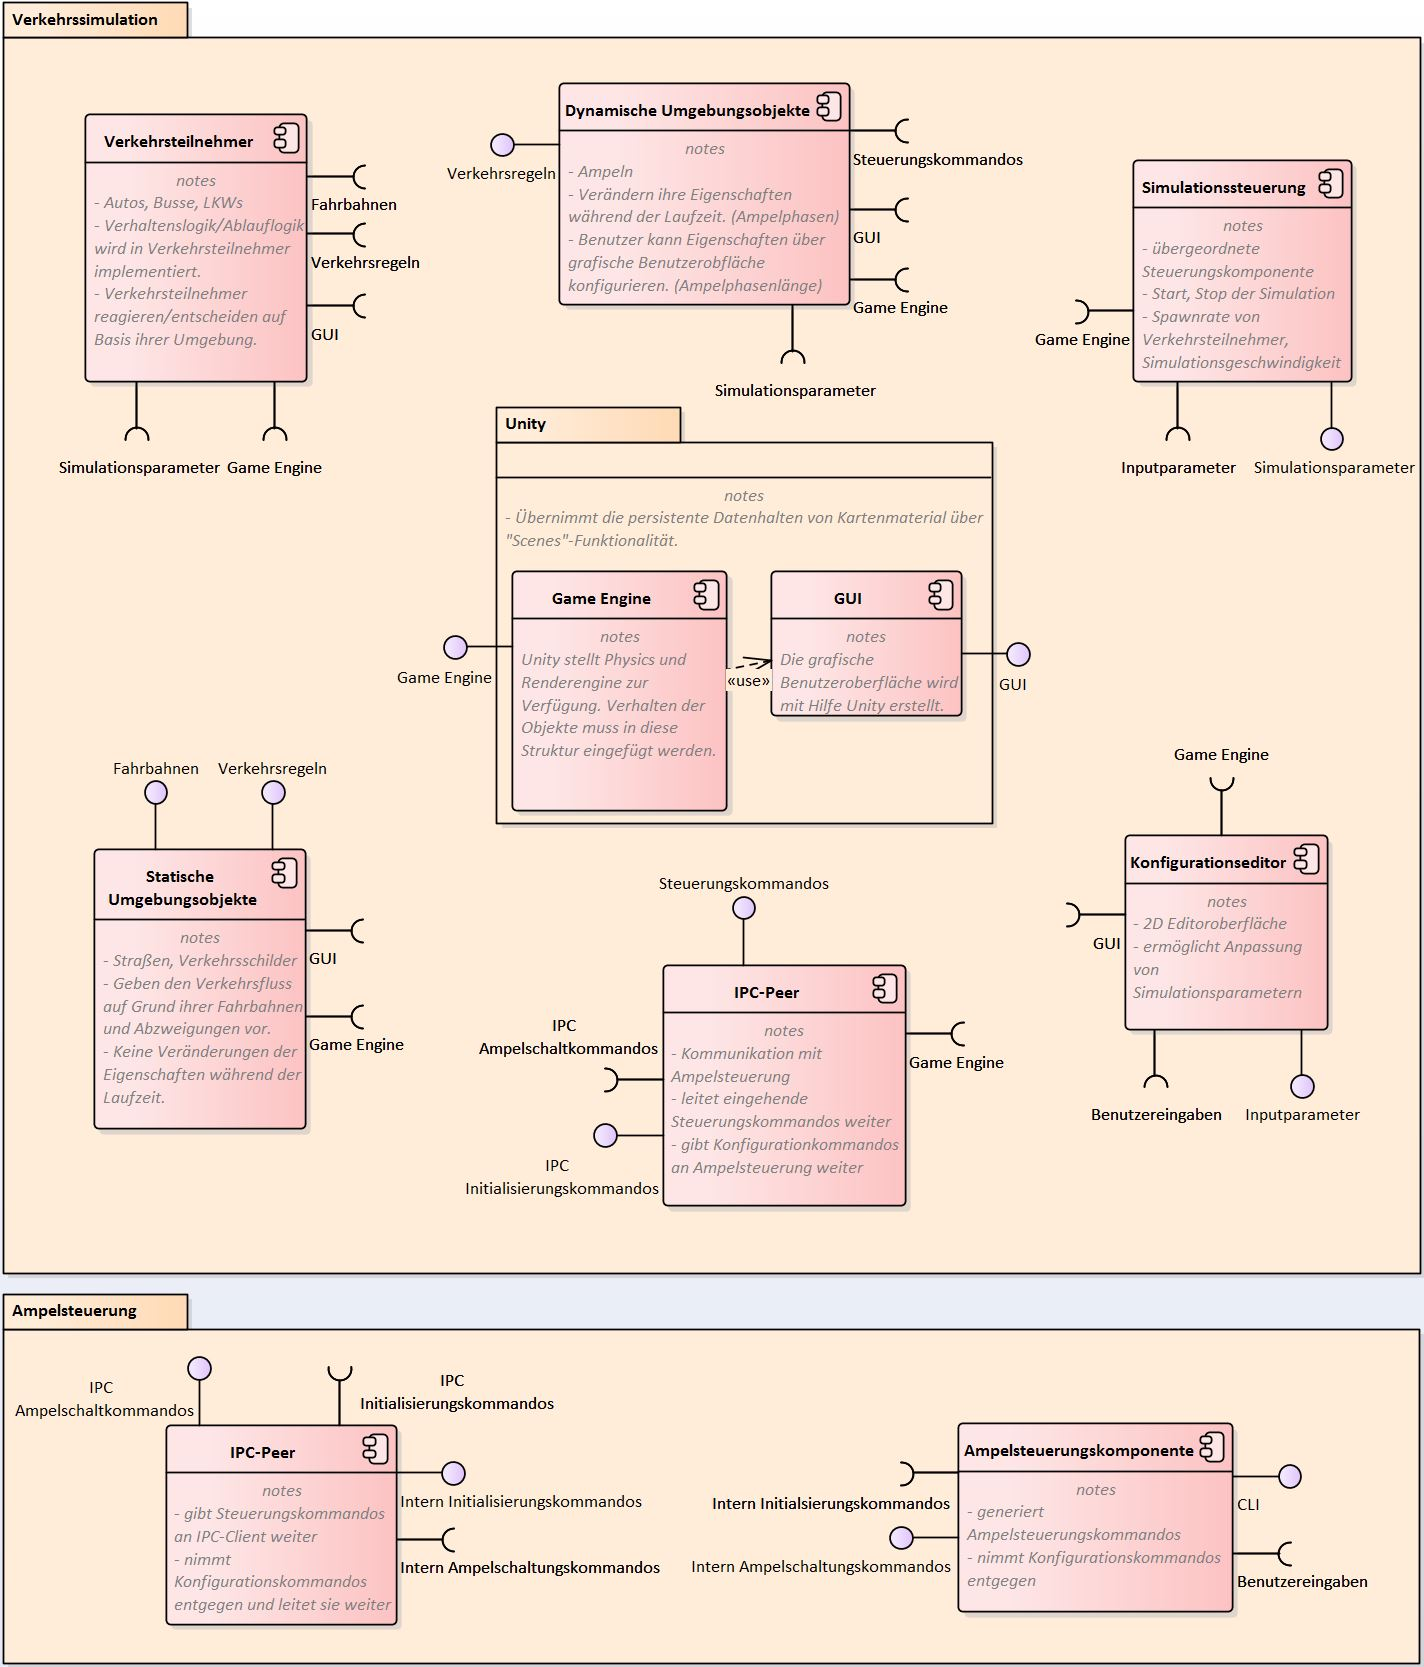
\includegraphics[scale=0.673]{BilderAllgemein/Komponentdiagram.JPG}
\end{center}
	%\includegraphics[width=\textwidth]
	%\end{center}
	% Title
	\caption{Komponenten Diagramm Verkehrssimulation}
	% Unique name: identifier for referencing
	%\label{Abbildung 2.1}
\end{figure}

\begin{flushleft}
\textbf{Verkehrssimulation und Ampelsteuerung}
\end{flushleft}
\vspace{-0.3 cm}

Sowohl Verkehrssimulation als auch Ampelsteuerung sind eigene Executables. Die Verkehrssimulation wird aus dem Unity-Projekt erzeugt und beinhaltet alle oben angegebenen Komponenten. Die Ampelsteuerung ist eine Konsolen Applikation, welche über die IPC-Komponenten mit der Verkehrssimulation kommuniziert.

\begin{flushleft}
\textbf{Verkehrsteilnehmer}
\end{flushleft}
\vspace{-0.3 cm}

Zu diesen Komponenten gehören alle sich aktiv in der Simulation bewegenden Objekte, wie Autos, Busse und LKWs. Die einzelnen Komponenten bewegen sich autonom voneinander im Straßennetz fort. Die Komponenten scannen ihre Umgebung auf Fahrbahnen, Verkehrsregeln und andere Verkehrsteilnehmer. Auf Basis dieses Scans entscheiden sie ihre nächste Aktion, wie zum Beispiel Beschleunigen, Bremsen oder Abbiegen. Verkehrsteilnehmer können sich ausschließlich auf Fahrbahnen bewegen und beachten alle Verkehrsregeln innerhalb ihres Aktionsradius. Weiters benötigen sie Simulationsparameter, die über ihre maximale Geschwindigkeit, Beschleunigung und Bremsverhalten entscheiden. Verkehrsteilnehmer treffen ihre Entscheidungen bei jedem Renderdurchlauf der Game Engine. Die Verknüpfung der Verkehrsteilnehmer mit der GUI erfolgt abstrahiert durch Unity.

\begin{flushleft}
\textbf{Dynamische Umgebungsobjekte}
\end{flushleft}
\vspace{-0.3 cm}

Dynamische Umgebungsobjekte sind Objekte, welche während der Simulationslaufzeit ihre Eigenschaften ändern, jedoch nicht ihre Position. Konkret sind dynamische Umgebungsobjekte Ampeln. Ampeln bieten den umliegenden Verkehrsteilnehmern ihren derzeitigen Status als Verkehrsregeln an, welche diese beachten müssen. Dynamische Elemente benötigen Simulationsparameter, welche ihre Schaltzeiten vorgeben. Konkret geben die Simulationsparameter die Phasenzeiten der Ampeln an. Weiters benötigen dynamische Umgebungsobjekte Steuerungskommandos um zwischen diversen Modi zu wechseln. Über Steuerungskommandos können Ampeln von automatischen Betrieb in einen inaktiven dauerhaft Gelb blinkenden Status gebracht werden. In jedem Renderzyklus der Game Engine wird auf neue Steuerungskommandos geprüft und falls nötig der vorgegebene Schaltvorgang eingeleitet. Die Verknüpfung der dynamischen Umgebungsobjekte mit der GUI erfolgt abstrahiert durch Unity.

\begin{flushleft}
\textbf{Simulationssteuerung}
\end{flushleft}
\vspace{-0.3 cm}

Die Simulationssteuerung stellt eine übergeordnete Kontrollinstanz der Simulation dar. Sie legt globale Einstellungen für Simulationskomponenten zentral fest. Die Simulationssteuerung bietet Simulationsparameter für andere Simulationskomponenten an, welche diese abrufen können. Konkrete Simulationsparameter sind Schaltzeiten für Ampeln, Höchstgeschwindigkeiten für Verkehrsteilnehmer oder Spawnraten für neue Verkehrsteilnehmer. Die Simulationssteuerung benötigt Inputparameter, welche von außen die Simulationsparameter bestimmen. Die Aktualisierung der Simulationsparameter auf Basis der Inputparameter erfolgt bei jedem Renderzyklus der Game Engine.

\begin{flushleft}
\textbf{Konfigurationseditor}
\end{flushleft}
\vspace{-0.3 cm}

Der Konfigurationseditor stellt eine zweidimensionale graphische Benutzeroberfläche dar, welche es dem Benutzer ermöglicht angebotene Inputparameter für die Simulation zu verändern. Vom Benutzer geänderte Inputparameter werden bei jedem Renderzyklus der Game Engine verarbeitet und entsprechend weiter geleitet.

\begin{flushleft}
\textbf{IPC-Peer Verkehrssimulation}
\end{flushleft}
\vspace{-0.3 cm}

Der IPC-Peer Verkehrssimulation repräsentiert eine Instanz der Inter Process Communication zwischen den Executables Verkehrssimulation und Ampelsteuerung dar. Dieser IPC-Peer gibt Initialisierungskommandos an die Ampelsteuerung weiter. Über diese Kommandos werden die benötigte Anzahl an Ampeln mit den korrekten Initialisierungsparametern angelegt. Weiters werden Ampelschaltkommandos entgegen genommen und weiter geleitet um den Modus einer Ampel zu wechseln. Ein- und ausgehende Kommandos während in jedem Renderzyklus der Game Engine bearbeitet.

\begin{flushleft}
\textbf{Statische Umgebungsobjekte}
\end{flushleft}
\vspace{-0.3 cm}

Statische Umgebungsobjekte repräsentieren Simulationskomponente, welche weder ihre Eigenschaften noch ihre Position während der Simulationslaufzeit verändern. Konkret sind Straßen und Verkehrsschilder statische Umgebungsobjekte. Sie bieten Fahrbahnen für die Verkehrsteilnehmer an, auf welchen diese sich bewegen können. Zusätzlich werden auch Verkehrsregeln vorgegeben, welche von den Verkehrsteilnehmer beachtet werden müssen. Die statischen Umgebungsobjekte werden von der Game Engine gerendert, jedoch sollte diese Komponente keine Logik besitzen. Die Verknüpfung der statischen Umgebungsobjekte mit der GUI erfolgt abstrahiert durch Unity.

\begin{flushleft}
\textbf{IPC-Peer Ampelsteuerung}
\end{flushleft}
\vspace{-0.3 cm}

Die Komponente IPC-Peer Ampelsteuerung bildet die Gegenstelle der zuvor beschriebenen IPC-Peer Verkehrssimulation. Sie gibt Ampelschaltkommandos zur Gegenstelle weiter und nimmt Initialisierungskommandos entgegen. Diese Kommandos werden intern, innerhalb der Ampelsteuerung Executable an die Ampelsteuerungskomponente weiter gegeben.

\begin{flushleft}
\textbf{Ampelsteuerungskomponente}
\end{flushleft}
\vspace{-0.3 cm}

Die Ampelsteuerungskomponente übernimmt die Verwaltung der einzelnen Ampelinstanzen. Anhand eingehender Initialisierungskommandos werden Ampelinstanzen mit den benötigten Initialisierungsparametern erstellt. Über das angebotene CLI kann der Benutzer Schaltbefehle absetzen, welche über Ampelschaltungskommandos weiter geleitet werden.

\begin{flushleft}
\textbf{Message Queue}
\end{flushleft}
\vspace{-0.3 cm}

Die Message Queue übernimmt die Kommunikation mit den anderen Gruppen. Die Kommunikation mit den anderen Gruppen wird über einen externen Server abgewickelt, auf denen sich die Gruppen anmelden und ihre Queues abonnieren können. Ein Format, basierend auf JSON wurde zwischen den Gruppenteilnehmern definiert.

Als Protokoll wird dabei AMPQ verwendet, der dazugehörende Server, RabbitMQ implementiert diese Protokoll und ermöglicht die Übertragung von Nachrichten.

\section{Laufzeitsicht}
\label{Laufzeitsicht}

Zur Laufzeit

\section{Verteilungssicht}
\label{Verteilungssicht}

\section{Querschnittliche Konzepte}
\label{Querschnittliche Konzepte}

Straßen und Kreuzungen werden als GameObjects abgespeichert. Dadurch wird ermöglicht, dass die erstellten Teilstücke wiederverwendet werden können. Somit kann die Erstellung der Welt per "Drag \& Drop" und genaues Ausrichten erfolgen. Folgende Straßenstücke wurden in verschiedenen Längen erstellt:

\begin{itemize}  
\item T-Kreuzung (mit Ampeln)
\item X-Kreuzung (mit Ampeln)
\item Spawn/Despan-Zone
\item Gerade Teilstrecke (5m, 6m, 24m, 30m, 40m, 50m, 60m)
\item 90 Grad Kurve
\end{itemize}

Die damit wiederverwendbaren Teilstücke beinhalten bereits die benötigten Kollider, welche für die Fahrzeuglogik verwendet werden, sowie Shaders zum Darstellen der Straßenstücke.

Auch das verwenden der Ampelsteuerung funktioniert über eine definierte Schnittstelle. Hierbei können einfach neue Kreuzungen mit Ampeln erstellt werden und die Ampelsteuerung regelt automatisch die neu erstellte Ampel.

\section{Entwurfsentscheidungen}
\label{Entwurfsentscheidungen}

Wie in Kapitel \ref{Lösungsstrategie} bereits kurz beschrieben wurde die Unity Engine als treibende Engine verwendet, da diese bereits viele Sachen implementiert, welche von uns nicht mehr berücksichtigt werden müssen (z.B. Handling wann wird welches GameObject angesprochen usw.). Ein weiterer Grund für die Entscheidung mit Unity war die schnelle und anschauliche Darstellung von 3D-Modellen, sowie die zahlreich vorhandenen Tutorials über Unity und die verschiedenen Möglichkeiten.

\section{Qualitätsszenarien}
\label{Qualitätsszenarien}

Keine Vorhanden, da es sich hierbei nur um ein Studierendenprojekt handelt.

\section{Risiken und technische Schulden}
\label{Risiken und technische Schulden}

Da die Verkehrssimulation nun zur Genze mit der Unity-Engine funktioniert, kann des im Falle von Updates von Unity vorkommen, das API-Updates durchgeführt werden und diese nicht mehr mit den bereits eingebauten funktionierenden Funktionen übereinstimmen. Dieses führt daraufhin zu Mehraufwand, der berücksichtigt werden müsste.
% !TeX root = Trafficsimulation_Documentation.tex

\chapter{Design}
\label{Design}

In diesem Kapitel werden die Implementierungen der einzelnen Komponenten sowie deren Schnittstellen zu anderen Komponenten dokumentiert.

% In diesem Kapitel das Design der Verkehrssimulation erklärt. Hier wird auf die wesentlichen Teile eingegangen, welche zum Erreichen der jeweiligen Ziele notwendig sind. 

% wos ghead hin?

\thispagestyle{standard}
\pagestyle{standard}

\section{Strassensystem}
\label{Strassensystem}

\subsection{Ampeln}

Die Ampeln wurden von uns als eigenständiges System geplant und umgesetzt. Um dieses Ziel zu erreichen erstellten wir zuerst auf Basis der Technologie TCP-Channel ein RemoteObject in Form einer eigenen DLL. Dieses RemoteObject definiert die Datenstrukturen, welche in weiterer Folge zwischen Client und Server geteilt werden. Als Serveranwendung erstellten wir eine Konsolenanwendung, welche wir auf einem öffentlich erreichbaren Linux Server mit Hilfe von Mono deployten. Als Clientgegenstellen für dieses System können verschiedene Unityinstanzen den Dienst der Serveranwendung verwenden. Sowohl am Client als auch am Server ist als DLL das RemoteObject hinterlegt. Instanzen des RemoteObjects können mit Hilfe am Server definierten Interfaces von den Clients erstellt und bearbeitet werden. Die somit erstellten Instanzen werden dann durch die TCP-Channel Technologie zwischen Client unser Server geteilt. Somit können Clients komfortabel mit ihrem lokalen Stub des RemoteObjects arbeiten ohne die Komplexität der IPC mitzubekommen. 

Durch die zentrale Definition des RemoteObjects in Form einer DLL können die geteilten Datenstrukturen zentral erweitert und gewartet werden.

\subsection{Straßen}

Das Design der einzelnen Straßenstücke wurde an den beiden Enden mit Collidern ausgestattet um somit ein durchgängiges Straßensystem erzeugen zu können, dem Autos folgen und dabei auf ihrer richtigen Spur bleiben.

\begin{figure}[H]
\begin{center}
	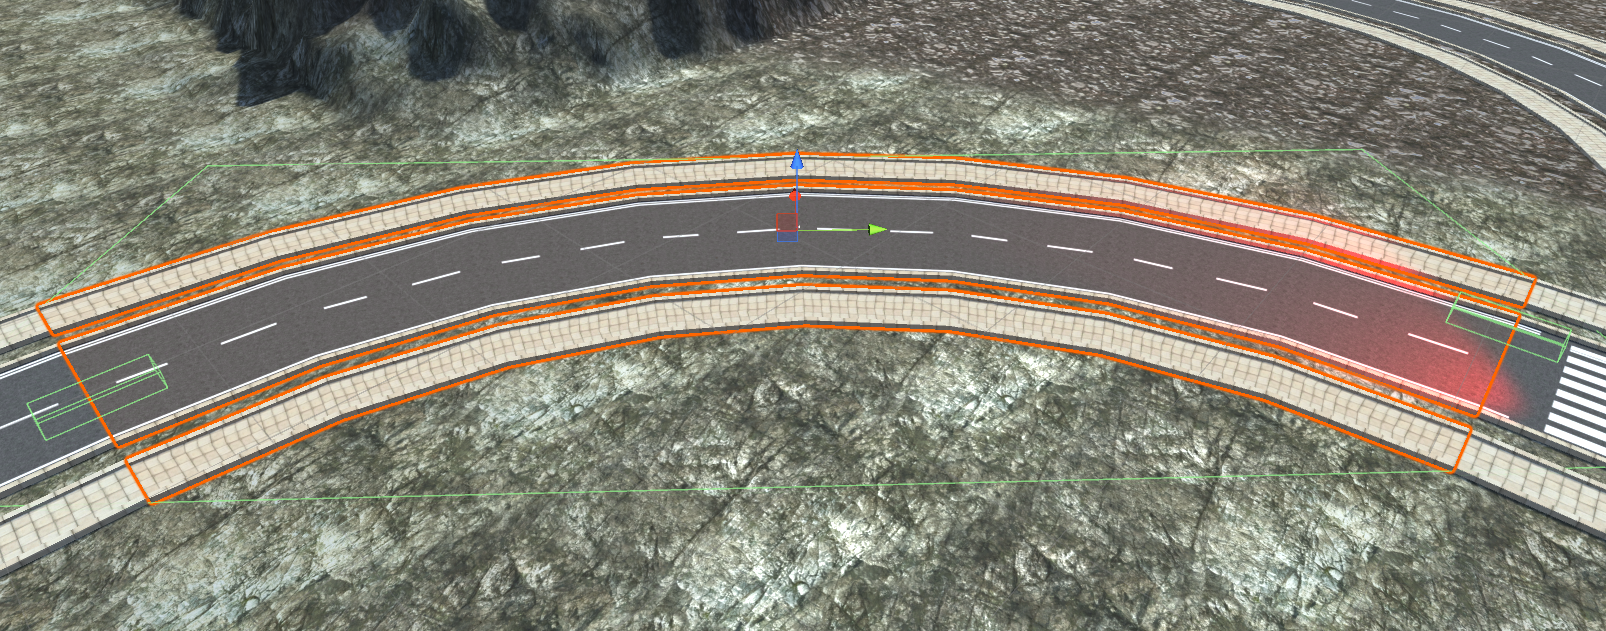
\includegraphics[width=1\textwidth]{BilderAllgemein/street_collider.png}
\end{center}
	\caption{Collider an normaler Straße}
	\label{img:street_collider}
\end{figure}

\subsection{Kreuzungen}

Die auf den Kreuzungen hinzugefügten Collider dienen dem jeweiligen Straßenabschnitt als Endpunkt an welchem sich die Fahrzeuge entscheiden müssen in welche Richtung sie weiterfahren wollen.

\begin{figure}[H]
\begin{center}
	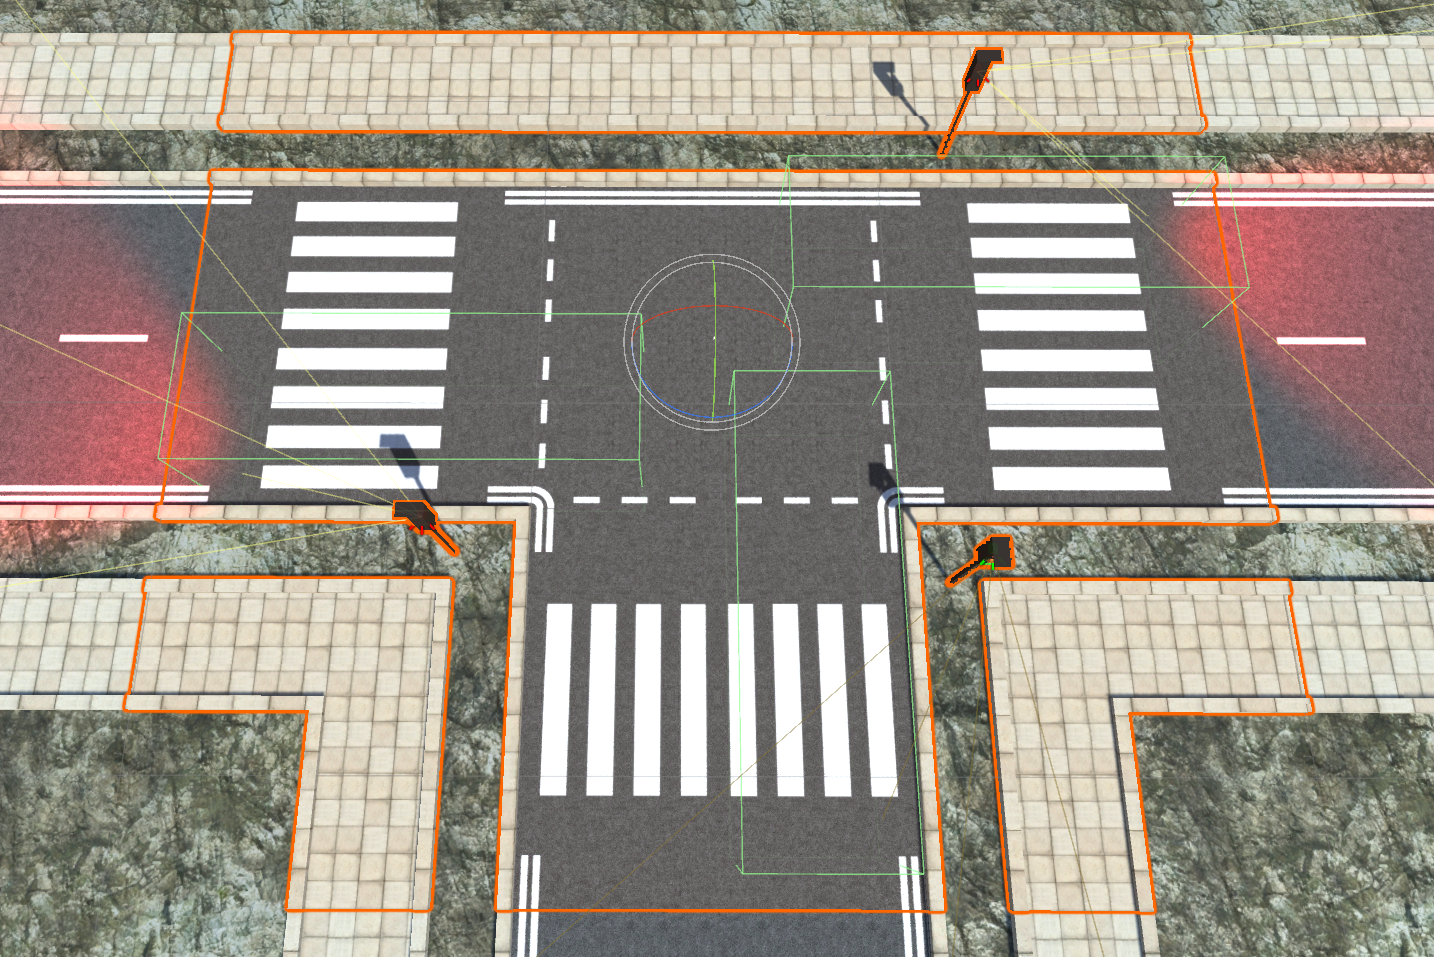
\includegraphics[width=1\textwidth]{BilderAllgemein/crossing_collider.png}
\end{center}
	\caption{Collider an Kreuzung}
	\label{img:crossing_collider}
\end{figure}

\subsection{Spawn}

Hier werden je nach Einstellung der Controls die Fahrzeuge gespawnt bzw despawnt, sobald sie mit dem in Abbildung \ref{img:spawn} gezeigten Collider in Berührung kommen.

\begin{figure}[H]
\begin{center}
	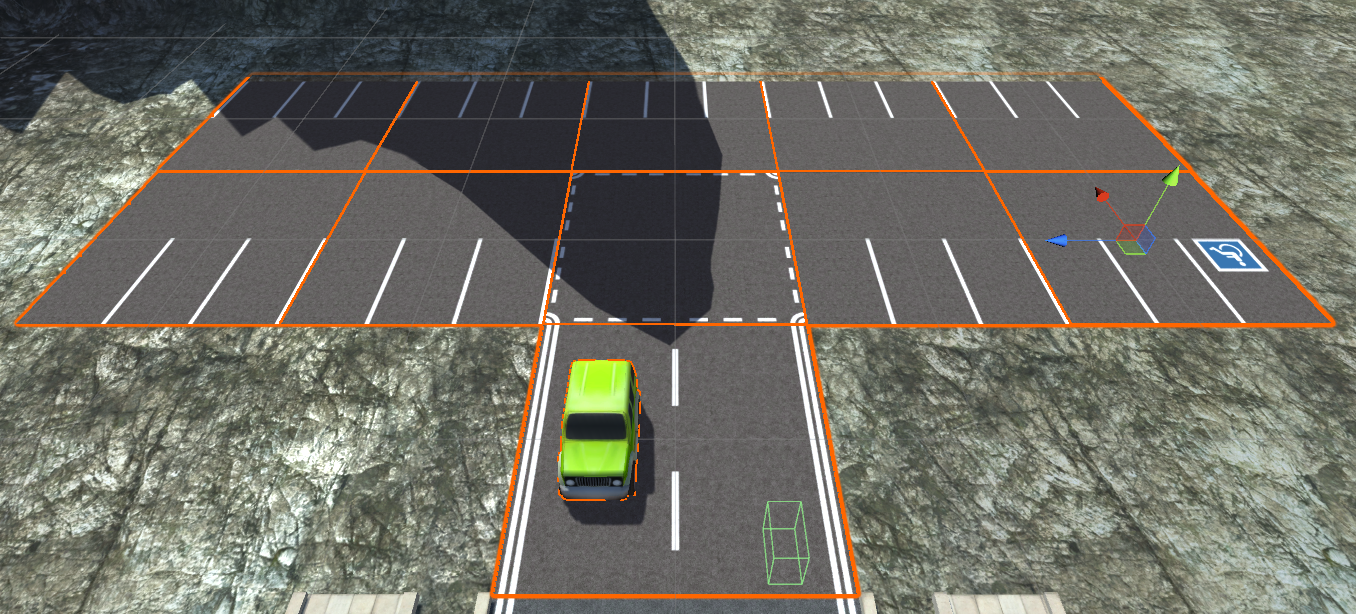
\includegraphics[width=1\textwidth]{BilderAllgemein/spawn.png}
\end{center}
	\caption{Spawn der Fahrzeuge}
	\label{img:spawn}
\end{figure}

\section{Fahrzeuglogik}
\label{Fahrzeuglogik}

Die Fahrzeuge implementieren alle ein Skript, welches für das Erkennen von Ampeln, Fahrzeugen und sonstiges Hindernissen zuständig ist. Dies ermöglicht eine völlige Kapselung und somit die Unabhängigkeit zur Straße und Kreuzung. Das bedeutet, dass Straßen und Kreuzungen nur sogenannte "Collider" zur Verfügung stellen, mit denen die Fahrzeuge interagieren können. Somit bleibt die gesamte Intelligenz in den Fahrzeugen.

Diese Collider werden je nach Geschwindigkeit des Fahrzeugs länger bzw. größer (wie in Abbildung \ref{img:car_collider} gezeigt) um somit auf Hindernisse wie andere Fahrzeuge, Kreuzungen und sonstiges frühzeitig reagieren zu können.

Das Erkennen und Verringern der Gschwindigkeit auf andere Fahrzeuge wird mittels Raycast erledigt. Die Lösung mit den Collidern war ein Problem, da sich die Fahrzeuge, nicht mehr bewegt haben, nachdem sie kollidiert sind.

\begin{figure}[H]
\begin{center}
	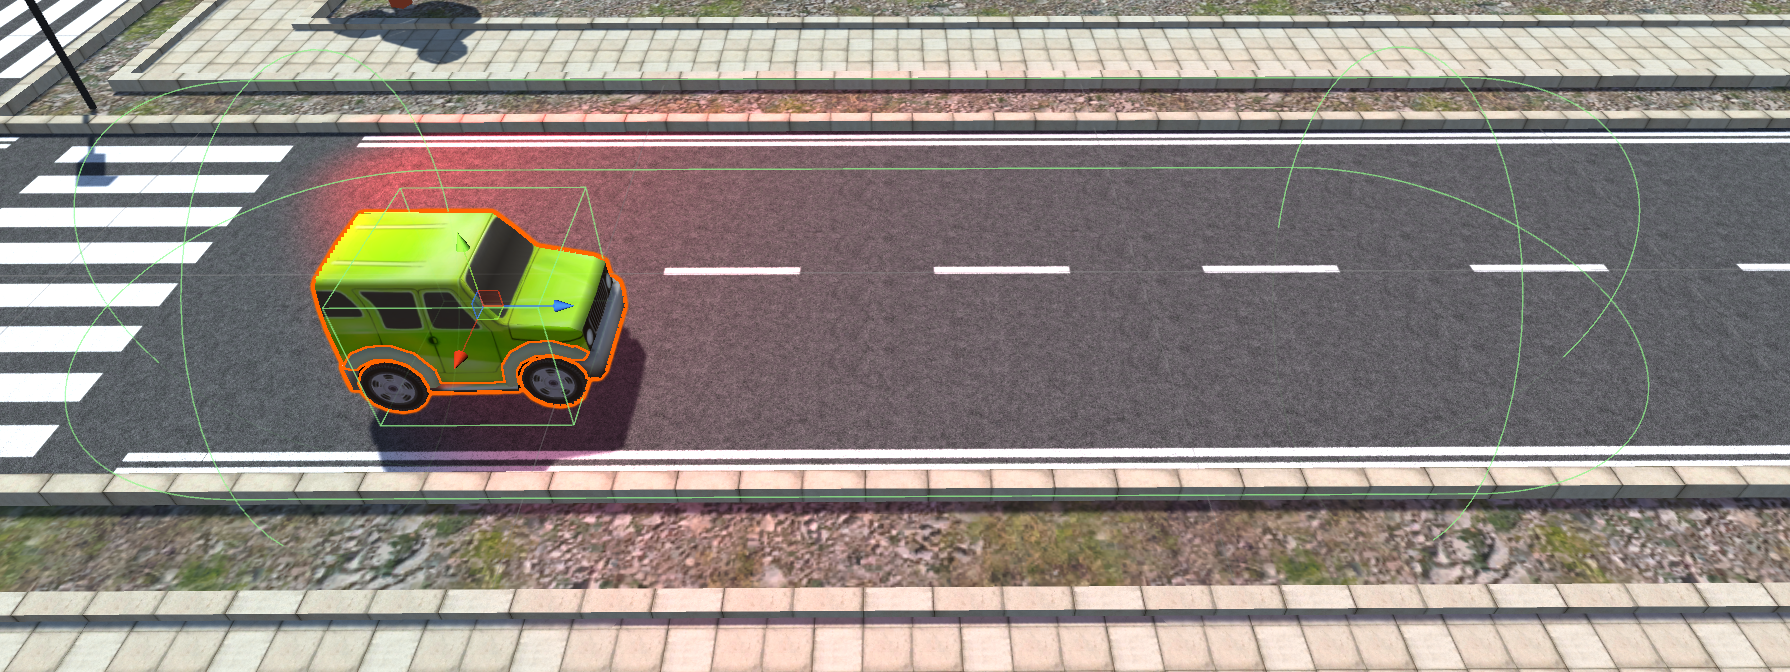
\includegraphics[width=1\textwidth]{BilderAllgemein/Jeep_Collider.png}
\end{center}
	\caption{Collider an Fahrzeugen}
	\label{img:car_collider}
\end{figure}

\section{Ampelsteuerung}

Die zentrale Komponente der Ampelsteuerung ist das RemoteObject. Wie bereits erwähnt handelt es sich dabei um eine eigenständige Komponente, welche in Form einer DLL in diverse Projekte leicht eingebunden und zentral gewartet werden kann. Das RemoteObject repräsentiert die Datenstrukturen und Funktionalitäten, welche zwischen Client und Server mit Hilfe der TCP-Channel Technologie geteilt werden.

Das RemoteObject bietet die Möglichkeit eine beliebige Anzahl von Kreuzungen zu erstellen und zu verwalten. Die Logik für den Aufbau der IPC-Verbindung wird dabei direkt im Client oder Server hinterlegt. Mit Hilfe von definierte Interfaces hat der Client die Möglichkeit Kreuzungen mit drei oder vier Ampeln am Server-Skeleton anzulegen. Die Kreuzungen werden entweder mit einer festgelegten Standardkonfiguration oder mit den vom Entwickler angegeben Übergabeparametern angelegt.

Von bereits angelegten Kreuzungen können die Zykluszeiten der einzelnen Ampeln editiert werden. Weiters ist es möglich das RemoteObject zu reseten und somit den Initialzustand wiederherzustellen.

Die einzelnen Kreuzungen, welche am RemoteObject angelegt sind können separat gestartet werden. Beim Starten einer Kreuzung wird ein eigener Thread für jede Ampel der Kreuzung erzeugt in dem eine Statemachine für die Ampelschaltung abläuft. Dieser Thread läuft bis entweder die Serveranwendung terminiert wird oder die Kreuzung durch einen Reset vom Client gelöscht wird. Die Statemachine einer Ampel durchläuft die üblichen Stati und berücksichtigt dabei die Konfiguration der entsprechenden Ampel. 

Mit Hilfe der ID einer Kreuzung und der Bezeichnung einer konkreten Ampel der Kreuzung kann der Status einer Ampel abgefragt werden.

Durch die Verwendung der TCP-Channel Technologie und der Definition des RemoteObjects in Form einer eigenen DLL wurde die Komplexität einer IPC sehr gut abstrahiert. Leider erfuhren wir während den Tests, dass die von uns verwendete Technologie sehr anfällig gegenüber schlechten Latenzzeiten ist. Dies wirkt sich in Form von Verbindungsproblemen zwischen Client und Server aus. Daher würde ich die Technologie TCP-Channel für IPC nur innerhalb eines lokalen Netzwerkes empfehlen.


\section{Hindernisse}
\label{Hindernisse}

Mit einem Klick der Maus sollen überall in der Welt Hindernisse platziert werden, welche anschließend von Fahrzeugen umfahren werden müssen. Durch einen weiteren Klick auf ein Hindernis soll dieses wieder gelöscht werden. 

Unity ermöglicht das Erstellen von GameObjects zur Laufzeit. Durch den Klick auf die Welt können die Koordinaten des Klicks festgestellt werden und somit das GameObject, welches bereits beim Start der Verkehrssimulation geladen wurde, platziert werden.

Durch das Halten eines Buttons auf der Tastatur soll die Erstellung von Hindernissen aktiviert werden. Dies verhindert, dass der Benutzer unbeabsichtigt zu viele Hindernisse erstellt.

\section{Aus- und Einfahren von Fahrzeugen anderer Gruppen}

Die Message Queue übernimmt die Kommunikation mit den anderen Gruppen. Die Kommunikation mit den anderen Gruppen wird über einen externen Server abgewickelt, auf denen sich die Gruppen anmelden und ihre Queues abonnieren können. Ein Format, basierend auf JSON wurde zwischen den Gruppenteilnehmern definiert.

Als Protokoll wird dabei AMPQ verwendet, der dazugehörende Server, RabbitMQ implementiert diese Protokoll und ermöglicht die Übertragung von Nachrichten.
% !TeX root = Trafficsimulation_Documentation.tex

\chapter{Implementierung}
\label{Implementierung}

In diesem Kapitel werden die Implementierungen der einzelnen Komponenten sowie deren Schnittstellen zu anderen Komponenten dokumentiert.

\thispagestyle{standard}
\pagestyle{standard}

\section{Erstellung der Welt}
\label{Erstellung_der_Welt}

\section{Fahrzeugsteuerung}
\label{Fahrzeugsteuerung}
% Inklusive Abbiegen, Weg folgen, Spawn

\section{Erkennen und Reagieren auf Ampeln}
\label{Erkennen_und_Reagieren_auf_Ampeln}

Das Event 'OnTriggerEnter' wird beim kollidieren mit Collidern generiert. In diesem Event, welches im 'FollowWay.cs' Skript implementiert wurde, wird überprüft, zu wem der kollidierte Collider gehört. Wird hierbei ein Ampelcollider erkannt, so wird dieser zwischengespeichert, sonst werden noch die anderen Collider auf der Kreuzung erkannt und es kommt zum Fehlverhalten im Fahrzeug. Die Bezeichnungen 'PosX', 'NegX', 'PosY' und 'NegY' beschreiben hierbei die Ampelpositionen.

\begin{lstlisting}[caption={Erstes erkennen einer Ampel},label={lst:ampel_erkennen}]
void OnTriggerEnter(Collider collider)
{
	GameObject itself = gameObject;
	GameObject colliededObject = collider.gameObject;

	float distance = getDistance(itself, colliededObject);
	if((colliededObject.name.Equals("PosX") ||
		colliededObject.name.Equals("NegX") ||
		colliededObject.name.Equals("PosY") ||
		colliededObject.name.Equals("NegY")) && (firstCollider == null))
	{
		//Here the car collided with a crossing collider
		crossingCurrent = collider.transform.parent.gameObject.transform.parent.gameObject; //The current crossing?!
		firstCollider = colliededObject;
	}
}
\end{lstlisting}

Nun wird das Event 'OnTriggerStay' aufgerufen, da sich das Fahrzeug immer noch im Collider der Ampel befindet. In diesem Event wird zwischen den zwei verschiedenen Kreuzungstypen, T- und X-Kreuzung unterschieden. Von diesen Kreuzungen wird sich dann eine Referenz geholt und den aktuellen Status der Ampel abgefragt. Je nach Status der Ampel verhält sich das Fahrzeug anders. Diese Verhalten wird in der 'carDecisionOnCrossing' Funktion festgelegt. Folgende Ampelverhalten wurden festgelegt:

\begin{itemize}  
\item \textbf{Grün:} Beschleunigen
\item \textbf{Blinkend Grün:} Beschleunigen
\item \textbf{Gelb:} Bremsen
\item \textbf{Blinkend Gelb:} Geschwindigkeit beibehalten
\item \textbf{Rot Gelb:} Beschleunigen
\item \textbf{Rot:} Bremsen
\end{itemize}

\begin{lstlisting}[caption={Bestehende Kollision mit Ampelcollider},label={lst:ampel_decision}]
void OnTriggerStay(Collider collider)
{
	GameObject collidedObject = collider.gameObject;

	if(collidedObject.name.Equals("PosX") ||
	collidedObject.name.Equals("NegX") ||
	collidedObject.name.Equals("PosY") ||
	collidedObject.name.Equals("NegY"))
	{
		CrossingColliderT crossT = null;
		CrossingColliderX crossX = null;

		float distance = getDistance(gameObject, collidedObject);
		if(collidedObject == firstCollider)
		{
			crossT = collidedObject.GetComponentInParent<CrossingColliderT>();
			if(crossT == null)
			{
				crossX = collidedObject.GetComponentInParent<CrossingColliderX>();
				if(crossX == null)
				{
					return;
				}
				RemoteObject.Enum.TrafficLightsStatus trafficLightStatus = crossX.actLightState;
				carDecisionOnCrossing(trafficLightStatus, distance);
			}
			else
			{
				RemoteObject.Enum.TrafficLightsStatus trafficLightStatus = crossT.actLightState;
				carDecisionOnCrossing(trafficLightStatus, distance);
			}
		}
	}
}
\end{lstlisting}

Die an den Fahrzeugen sitzenden Collider werden in jedem Update Aufruf je nach Geschwindigkeit des Fahrzeuges vergrößert bzw. verkleinert, so kann auf Ampeln hingebremst werden und kein abruptes Stehenbleiben erzwungen werden.

\section{Fahrzeug Kollisionserkennung}
\label{Fahrzeug_Kollisionserkennung}

Jedes Fahrzeug implementiert das 'FollowWay.cs' Skript welches die komplette Logik über das Verkehrsverhalten besitzt. Innerhalb dieses Skripts wird in der Update-Methode, welche in jedem Frame pro Sekunde aufgerufen wird, überprüft, ob ein Raycast mit einem anderen Fahrzeug oder Hindernis kollidiert ist. Da dieser Raycast mehrere Objekte durchdringen kann, muss in einer Liste überprüft werden ob mit einem dieser Objekte kollidiert werden soll. Ist dies der Fall, so wird die Geschwindigkeit des Fahrzeugs verringert und der Raycast wird auf die Länge, welche der Geschwindigkeit des Fahrzeugs entspricht, gesetzt. Dazu wird die Distanz des zu kollidierenden Objekts und dem Fahrzeug ermittelt. Mit der Distanz wird das Fahrzeug dann entsprechend abgebremst und wenn nötig auch zum Stillstand gebracht. Um nicht in das vorherfahrende Objekt zu fahren, wird die Hälfte der Länge des Fahrzeugs noch von der Distanz abgezogen. Damit sich das Fahrzeug nicht selbst als kollidierendes Objekt erkennt, muss der Layer des Fahrzeugs für kurze Zeit geändert werden.

\begin{lstlisting}[caption={Erkennen von anderen Fahrzeugen und Hindernissen},label={lst:Hinderniss_erkennen}]
private void checkRaycast()
{
	// Save current object layer
	int oldLayer = gameObject.layer;
	//Change object layer to a layer it will be alone
	gameObject.layer = 12;
	int layerToIgnore = 1 << 12;
	layerToIgnore = ~layerToIgnore;

	RaycastHit[] hits;		
	hits = Physics.RaycastAll(transform.position, transform.forward, raycastSize, layerToIgnore);
	bool somethingInFront = false;
	for(int i = 0; i < hits.Length; i++)
	{
		RaycastHit hit = hits[i];
		GameObject collidedObject = hit.collider.gameObject;
		if(collidedObject.name.Equals("jeep(Clone)") || collidedObject.name.Equals("Rock(Clone)"))
		{
			float distance = getDistance(gameObject, collidedObject);
			if(gameObject.name.Equals("jeep(Clone)"))
			{
				distance = distance - (lengthCar / 2 + 1f);
			}
			else
			{
				distance = distance - (lengthTanker / 2 + 1f);
			}
			brakeWithDistance(distance);
			mayIdrive = false;
			somethingInFront = true;
		}
		if(somethingInFront == false)
		{
			mayIdrive = true;
		}
	}
	raycastSize = speed;
	if(raycastSize < 1)
	{
		raycastSize = 1;
	}
	// set the game object back to its original layer
	gameObject.layer = oldLayer;
}
\end{lstlisting}

\section{Ampelsteuerung}
\label{Ampelsteuerung}

Die Ampelsteuerung wurde als eigene Applikation entwickelt. Die Ampelsteuerung kann grundsätzlich unabhängig von der Unity-Spielwelt laufen, auch die Ampeln schalten dementsprechend autonom, auch wenn die Simulation schon beendet sein sollte.

%... evtl. mike wos

Die Ampelsteuerung ist auch mit Mono lauffähig. Mono ist eine C\#-Implementierung für unixoide Betriebssysteme. So läuft die Ampelsteuerung auch mit Linux. Auch eine Kompilierung ist möglich, mit \texttt{xbuild solution.sln} wird eine ausführbare Datei erzeugt, die sowohl mit Linux als auch Windows lauffähig ist.

In Abbildung \ref{img:ampel} ist die Ausgabe der Ampelsteuerung zu sehen. Da die Ampelsteuerung gut funktionierte, wurde in die Ausgabe weniger Zeit investiert, sodass hier nur die aufrufende IP ausgegeben wird.

\begin{figure}[H]
\begin{center}
	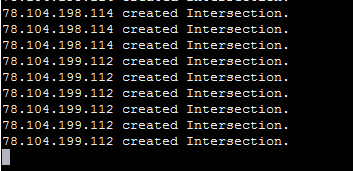
\includegraphics[width=0.65\textwidth]{BilderAllgemein/ampelserver.png}
\end{center}
	\caption{Ausgabe Ampelserver}
	\label{img:ampel}
\end{figure}

\section{Erstellen und Löschen von Hindernisse}

Um im Environment Hindernisse zur Laufzeit zu Erstellen, muss dem Terrain-GameObject ein Skript (Obstacles.cs) hinzugefügt werden. In diesem Skript findet die Abarbeitung des Inputs des Users statt.

Wie bereits in \ref{Hindernisse} erläutert wird zum Start der Verkehrssimulation das Hindernis geladen. Dies erfolgt über den "Load" Befehl.

\begin{lstlisting}[caption={Laden des Hindernisses},label={lst:Hinderniss_laden}]
private GameObject prefabLog;
void Start()
{
	prefabLog = Resources.Load("Rock", typeof(GameObject)) as GameObject;
}
\end{lstlisting}

Der in \ref{Hindernisse} beschrieben soll ein Button gedrückt gehalten werden um Hindernisse spawnen zu können. Dieser wird über einen KeyCode definiert. Im Skript wird nun in jedem Update Aufruf darauf gewartet, ob der definierte Button gedrückt und ein "MouseDown" Event vorkommt. Mit diesem Event kann die Position der Maus auf dem Bildschirm herausgefunden werden, jedoch stimmen diese nicht mit den Welt-Koordinaten überein. Deshalb muss hier eine Umwandlung durchgeführt werden, welche mit Hilfe eines Raycasts gelöst wurde. Durch das Instanzieren wird das neu erstellte Hindernis in der Welt platziert.

\begin{lstlisting}[caption={Erstellen des Hindernisses},label={lst:Hinderniss_erstellen}]
private KeyCode shiftLeft = KeyCode.LeftShift;
if(Input.GetMouseButtonDown(0) && Input.GetKey(shiftLeft)) //Left mouse button clicked
{
	Vector3 mousePosition = Input.mousePosition;
	var ray = Camera.main.ScreenPointToRay(mousePosition);
	RaycastHit hit;
	if(Physics.Raycast(ray, out hit, 1000f))
	{
		Vector3 position = hit.point;			Vector3 yOffset = new Vector3(0, 1.5f, 0);
		position += yOffset;			
		GameObject prefabInstance = Instantiate(prefabLog, position, new Quaternion()) as GameObject;
	}
}
\end{lstlisting}

Zum Löschen eines Hindernisses muss die rechte Maustaste in Kombination mit dem vorher definierten Button verwendet werden. Mittels "Destroy" wird anschließend das erkannte GameObject wieder von der Welt gelöscht.

\begin{lstlisting}[caption={Zerstören des Hindernisses},label={lst:Hinderniss_zerstören}]
if(Input.GetMouseButtonDown(1) && Input.GetKey(shiftLeft)) //Right mouse button clicked
{
	Vector3 mousePosition = Input.mousePosition;
	var ray = Camera.main.ScreenPointToRay(mousePosition);
	RaycastHit hit;
	if(Physics.Raycast(ray, out hit, 1000f))
	{
		Vector3 position = hit.point;
		GameObject collidedObject = hit.collider.gameObject;
		if(collidedObject.name.Equals("Rock(Clone)"))
		{
			Destroy(collidedObject);
		}
	}
}
\end{lstlisting}

\begin{figure}[H]
\begin{center}
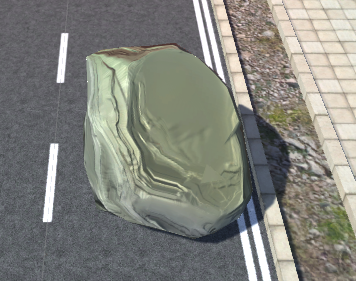
\includegraphics[width=0.5\textwidth]{BilderAllgemein/rock.PNG}
\end{center}
	\caption{Hindernis}
	\label{img:hindernis}
\end{figure}

\section{Aus- und Einfahren von Fahrzeugen anderer Gruppen}
\label{Aus-_und_Einfahren_von_Fahrzeugen_anderer_Gruppen}

Mit dem Plugin `Unity3D.Amqp` (\url{https://github.com/CymaticLabs/Unity3D.Amqp}) für Unity ist es möglich einen RabbitMQ-Server direkt in Unity einzubinden.

Die Konfiguration der Serverdaten werden dabei direkt in den Menüeinstellungen von Unity vorgenommen. Die verwendete Konfiguration ist in Abbildung \ref{img:rabbit} zu sehen.

\begin{figure}[H]
\begin{center}
	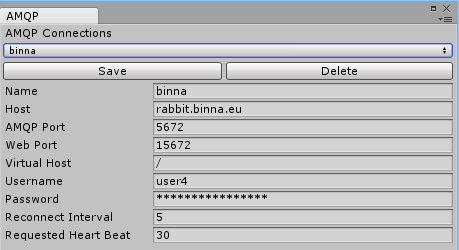
\includegraphics[width=0.9\textwidth]{BilderAllgemein/rabbitconfig.png}
\end{center}

	\caption{Einstellungen RabbitMQ}

	\label{img:rabbit}
\end{figure}

Jede Gruppe bekam einen eigenen Benutzer samt Passwort. Damit man Nachrichten empfangen kann, muss man sich auf eine `Queue` subscriben.

Das Plugin stellt anschließend Methoden zur Verfügung. Eine solche Methode ist \texttt{OnMessageReceived()}. Damit lässt sich eine eingehende Nachricht an ein Objekt in der Spielwelt weitergeben. Das Objekt kann daraufhin reagieren, beispielsweise ein Auto erzeugen.

\begin{figure}[H]
\begin{center}
	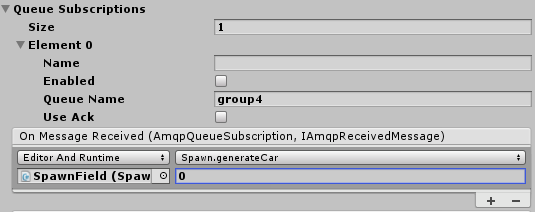
\includegraphics[width=0.9\textwidth]{BilderAllgemein/rabbitqueue.png}
\end{center}

	\caption{RabbitMQ Queue}

	\label{img:rabbitq}
\end{figure}

In Abbildung \ref{img:rabbitq} sieht man wie eine eingehende Nachricht beim Objekt \texttt{SpawnField} eine Methode aufruft.
% !TeX root = Trafficsimulation_Documentation.tex

\chapter{Review einer fremden Architekturdokumentation}
\label{Review_einer_fremden_Architekturdokumentation}

\thispagestyle{standard}
\pagestyle{standard}

In diesem Kapitel wird die Architekturdokumentation der Gruppe Binna/Dorfer/Gruber/Mühlbacher/Wieser überprüft.
Dazu wurde die uns zur Verfügung gestellte Version 8 vom 27.06.2017 reviewt. Als Hilfestellung wurden auch Vorgaben aus den im Labor erwähnten Podcasts und Dokumente zum Thema Architektur und Architektur-Reviews genutzt.

Als Grundlage für die Architekturdokumentation wurde das arc42 Template verwendet. Dadurch ließ sich beim Review leicht feststellen, wie weit die einzelnen Punkte der Vorlage erfüllt wurden, oder wo es Abweichungen gab.


Der Abschnitt Einführung und Ziele enthält die Aufgabenstellung und alle geforderten Ziele. Dabei werden diese einfach und verständlich dokumentiert. Detailliertere Beschreibungen folgen erst in den nächsten Abschnitten.


Die tabellarische Form der Anforderungen/Qualitätsziele/Stakeholder ergibt eine übersichtliche Zusammenfassung. Allerdings sind manche Punkte verteilt an mehreren Stellen im Dokument beschrieben und es könnten daher Dinge übersehen werden. z.B. "Der User soll gewisse Parameter die Simulation betreffend verändern können.". Welche Parameter genau veränderbar sein sollen, findet man aber woanders.


Auch bei den Rahmenbedingungen wurde eine Tabelle genutzt die sicherstellt, dass diese eindeutig vom Leser erkennbar sind.


Im fachlichen Teil des Abschnitts Kontextabgrenzung fehlt die Beschreibung des Use-Case Diagramms. Nicht mit dem Projekt vertraute Personen könnten dieses falsch interpretieren. Der technische Kontext ist aufgrund der vorhergehenden Beschreibung besser zu verstehen. Eventuell wäre es noch sinnvoll zu beschreiben, was das System NICHT erfüllen soll.


Die Lösungsstrategien sind teilweise identisch mit den Rahmenbedingungen und geben keine Wirkliche Strategie vor.
Außerdem verhindert die Aufzählungsform eine Begründung der einzelnen Punkte. Leser werden nicht darüber informiert wieso es zu den einzelnen Entscheidungen kam und könnten dieselben Fragen erneut Stellen.


Die Bausteinsicht ist übersichtlich gegliedert, indem sie in Ebenen mit verschiedenen Detailgraden unterteilt wird. Allerdings fehlt die Beschreibung zum Komponentendiagramm in der höchsten Ebene die als Übersicht über die einzelnen Komponenten für den Leser dienen soll. Gerade an dieser Stelle wären allgemeine Informationen und Beschreibungen wichtig. In der zweiten Ebene wurden die einzelnen Komponenten ausführlicher Beschrieben, allerdings fehlen einige technische Details in Textform (z.B. wie einzelne Schnittstellen technisch realisiert werden).


Grundsätzlich wurde in der Architekturdokumentation zu sehr davon ausgegangen, dass der Leser bereits über das Projekt informiert ist. Auf Hilfen wie Anforderungsschablonen oder Patterns wurde nicht zurückgegriffen. Laufzeit- und Verteilungssicht fehlen. Kurz vor dem Abgabetermin stand nur die Version 8 der Architekturdokumentation zur Verfügung. Das Review basiert daher nur auf den bis zu diesem Zeitpunkt dokumentierten Punkten des arc42 Templates.
%\include{DokumentPraktikumsbericht}
%\include{40PraktischeUmsetzungGISControl}
%\include{50RueckundAusblick}


%%%%%%%%%%%%%%%%%%%%%%%%%%%%%%%%%%%%%%%%%%%%%%%%%%%%%%%%%%%%%%%%%%%%%%%%%%%%%%%%%%%%%%%%%%%%%%%%%%%%%%%%%%%%
% LITERATURVERZEICHNIS

\interlinepenalty=10000 % Literatureinträge: Absätze zusammenhalten
\clearpage
\addcontentsline{toc}{chapter}{Literatur}
\singlespace
%\bibliography{12bibliografie}
%\bibliography{Literaturverzeichnis}
\interlinepenalty=100

%%%%%%%%%%%%%%%%%%%%%%%%%%%%%%%%%%%%%%%%%%%%%%%%%%%%%%%%%%%%%%%%%%%%%%%%%%%%%%%%%%%%%%%%%%%%%%%%%%%%%%%%%%%%
% ANHÄNGE

%\begin{appendix}
%\include{Anhang_Mathematik}                 % A
%\include{Anhang_FormatDerParameterdateien}  % B
%\include{Anhang_Quelltexte}                  % C
%\include{Anhang_Datenblaetter}              % D
%\include{Anhang_Glossar}                    % E
%\end{appendix}

\end{document}